% Lecture Template for ME3001-001-Tristan Hill - Spring 2020
% Mechanical Engineering Analysis with MATLAB
% Ordinary Differential Equations - Lecture 3

% I am finally converting my stuff to BEAMER

% Document settings



%\documentclass{beamer}                  % for presentation ?
\documentclass[handout]{beamer}  % for handout ?
\usepackage{beamerthemesplit}
\usepackage{amsmath}
\usepackage{listings}
\usepackage{multicol}

\beamertemplateballitem

\definecolor{TTUpurple}{rgb}{0.3098, 0.1607, 0.5176} % TTU Purple (primary)
\definecolor{TTUgold}{rgb}{1.0000, 0.8666, 0.0000} % TTU Gold (primary)

\setbeamercolor{palette primary}{bg=TTUpurple,fg=TTUgold}
\setbeamercolor{palette secondary}{bg=black,fg=TTUgold}
\setbeamercolor{palette tertiary}{bg=black,fg=TTUpurple}
\setbeamercolor{palette quaternary}{bg=TTUgold,fg=black}
\setbeamercolor{structure}{fg=TTUpurple} % itemize, enumerate, etc
\setbeamercolor{section in toc}{fg=TTUpurple} % TOC sections

% Override palette coloring with secondary

%\setbeamercolor{subsection in head/foot}{bg=TTUgold,fg=TTUpurple}

%\usefonttheme{professionalfonts}

\newcommand{\LNUM}{4\hspace{2mm}} % Lecture Number 
\newcommand{\secondtitle}{Validation of Analytical Solutions with ODE45}% second line of the title of this presentation , aka the topic of this lecture
\newcommand{\vspcc}{\vspace{6mm}\\ } 
\newcommand{\vspc}{\vspace{3mm}\\ } 
\newcommand{\hspc}{\hspace{5mm} } 


\title{\vspace{2mm}\\ Ordinary Differential Equations - Lecture \LNUM}
\author{ME3001 - Mechanical Engineering Analysis} % original formatting from Mike Renfro, September 21, 2004

\date{April 02, 2020}

\begin{document}

\lstset{language=MATLAB,basicstyle=\ttfamily\small,showstringspaces=false}


\frame{\titlepage \center\textbf{\secondtitle}\vspcc}
\frame{

{\bf Lecture \LNUM - \secondtitle:} \vspace{3mm}\\ % ' topics' are beamer 'sections' - TWH

 \begin{itemize}
	\item Review\vspace{5mm}\\
	\item Solution Validation \vspace{5mm}\\
	\item MATLAB ode45() function \vspace{5mm}\\		
	\item Example - 1986 (or 1968?) Ferrari Testarosa Spider \vspace{5mm}\\
\end{itemize}

}

\section{Review}

\subsection{Analytical vs. Numerical Methods}
\frame{

  \frametitle{Analytical vs. Numerical Methods}

{\bf Analytical solutions (methods)}, also called closed-form solutions, are mathematical solutions in the form of math expressions. If you are developing algorithms or modeling engineering systems, analytical solutions offer the advantages of transparency and efficiency. \vspace{2mm}\\

{\bf Numerical methods} for ordinary differential equations are methods used to find numerical approximations to the solutions of ordinary differential equations (ODEs). Their use is also known as "numerical integration", although this term is sometimes taken to mean the computation of integrals.

}

\section{Engineering Example - Validation of Analytical Solution}
\subsection{Engineering Example - Validation of Analytical Solution}
\frame{

\frametitle{Engineering Example - Validation of Analytical Solution}



Remember our example from the previous lecture?\vspace{5mm}\\

        \scalebox{1.25}{$m\dot{v}+cv=f(t) \hspace{5mm}\rightarrow\hspace{5mm} v(t)=(v_0-\frac{F}{c})e^{-\frac{c}{m}t}+\frac{F}{c}$} \vspace{5mm}\\
	
	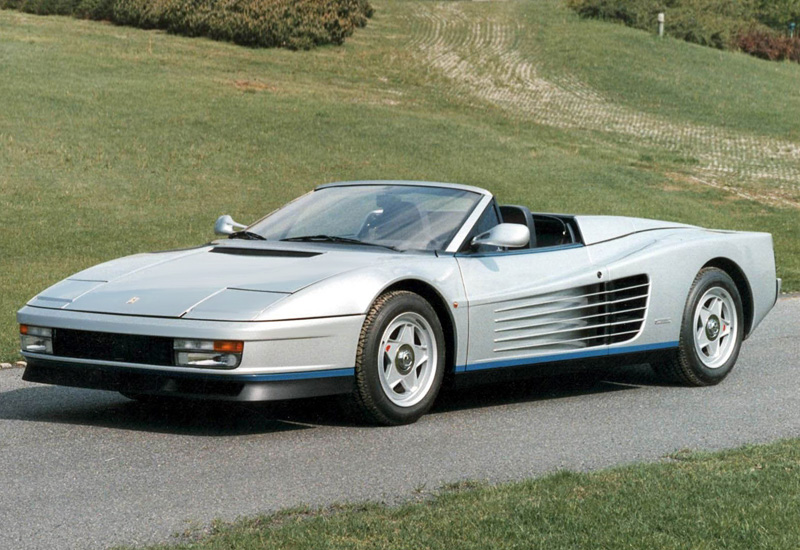
\includegraphics[scale=0.15]{ferrari.jpg} \hspace{10mm} 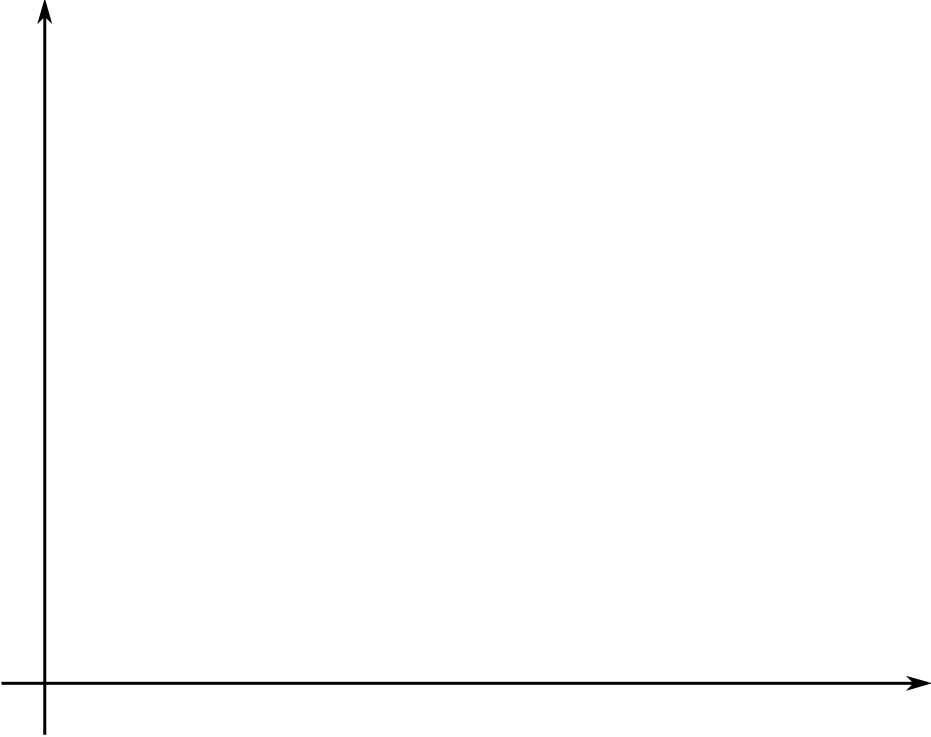
\includegraphics[scale=0.10]{lecture1_fig2.png}\vspace{5mm}\\
	
	
How do we know that the analytical solution we derived is correct? \vspace{10mm}\\
  

}

\section{Solution Validation}

\subsection{Solution Validation}
\frame{

  \frametitle{Solution Validation}

{\bf Q:} How do we know that the solution we derived is correct? \vspace{5mm}\\ 
{\bf A:} \vspace{10mm}\\

}

\section{ODE45 function in MATLAB}

\subsection{Use the Help References}

\frame[containsverbatim]{

  \frametitle{Use the Help References}

 
We are going to solve the differential same equation in {\it MATLAB} using the {\bf ode45} function. \vspace{3mm}\\
This {\it built-it} function uses {\bf numerical integration} to approximate a solution an ODE as an {\bf initial value problem}.\vspace{2mm}\\ 

  \begin{lstlisting}

  >> help ode45 
 
  \end{lstlisting}

\vspace{3mm} Use the help in the MATLAB command window or look it up elsewhere. It can be hard to understand.


}


\subsection{Using the ODE45 function}

\frame[containsverbatim]{

  \frametitle{Using the ODE45 function}

 
The {\bf ode45} function is a powerful tool and it is easy to use. \vspace{0mm}\\

  \begin{lstlisting}

[t_45,y_45]=ode45(@ODEFUN,TSPAN,Y0,OPTIONS,P...);
 
  \end{lstlisting}

\vspace{3mm} Here is a description of the arguments.\vspace{2mm}\\

ODEFUN - name of the function containing the model \vspace{2mm}\\
TSPAN - time range for the initial value problem \vspace{2mm}\\
Y0 - initial value of the dependent variable \vspace{2mm}\\
OPTIONS - options defined by OPTIMSET function \vspace{2mm}\\
P... - additional parameters passed to ODEFUN \vspace{2mm}\\


}


\subsection{Graph of the Solution}

\frame[containsverbatim]{

\frametitle{Graph of Solution}

Do the results from the two methods agree?\vspace{2mm}\\

\begin{lstlisting}

figure(1);hold on
plot(t_45,y_45)
 
  \end{lstlisting}
\vspace{30mm}


}
\end{document}









